\documentclass[../notes.tex]{subfiles}

\pagestyle{main}
\renewcommand{\chaptermark}[1]{\markboth{\chaptername\ \thechapter\ (#1)}{}}
\setcounter{chapter}{4}

\begin{document}




\chapter{Enolate Chemistry}
\setcounter{section}{28}
\section{Enols and Enolates}
\begin{itemize}
    \item \marginnote{11/15:}Grade cutoffs on Exam 3.
    \begin{itemize}
        \item A: 85-100.
        \item B: 70-84.
        \item C: 63-69.
        \item $<\text{C}$: $<57$.
        \item If you are considering dropping this class, the drop date is 11/20.
        \begin{itemize}
            \item It does not count as a drop if you just stop showing up and stop submitting assignments.
            \item Go to the Registrar's site and fill out an add/drop form.
        \end{itemize}
        \item If you are doing less well than you had hoped or expected, talk to your TFs about options!
        \begin{itemize}
            \item You may be eligible for tutoring.
            \item It is \emph{your responsibility} to reach out for help.
        \end{itemize}
    \end{itemize}
    \item Fun (or scary) Friday: Prof. Buchwald sings the elements song!
    \item Announcement: Unit 5 study guide posted.
    \item We now begin the first of four lectures in Unit 5: Enols and enolates.
    \begin{itemize}
        \item Readings: Chapters 20, 25, 26 of \textcite{bib:Clayden}.
    \end{itemize}
    \item Lecture outline.
    \begin{enumerate}[label={\Alph*.}]
        \item Background.
        \begin{itemize}
            \item Enolate definition.
            \item Keto-enol tautomerization (base-catalyzed and acid-catalyzed).
            \item Evidence: Deuterium exchange.
        \end{itemize}
        \item $\alpha$-halogenation of ketones.
        \begin{itemize}
            \item Base-promoted mechanism (and complications).
            \item The iodoform reaction.
            \item Acid-catalyzed mechanism.
        \end{itemize}
        \item $\alpha$-alkylation.
        \begin{itemize}
            % \item General form.
            \item Lithium diisopropylamide.
            \item Malonate ester synthesis.
            \item Kinetic vs. thermodynamic enolates.
        \end{itemize}
    \end{enumerate}
    \pagebreak
    \item We'll begin with Topic A: Background.
    \item Defining enolates.
    \begin{figure}[h!]
        \centering
        \begin{subfigure}[b]{0.4\linewidth}
            \centering
            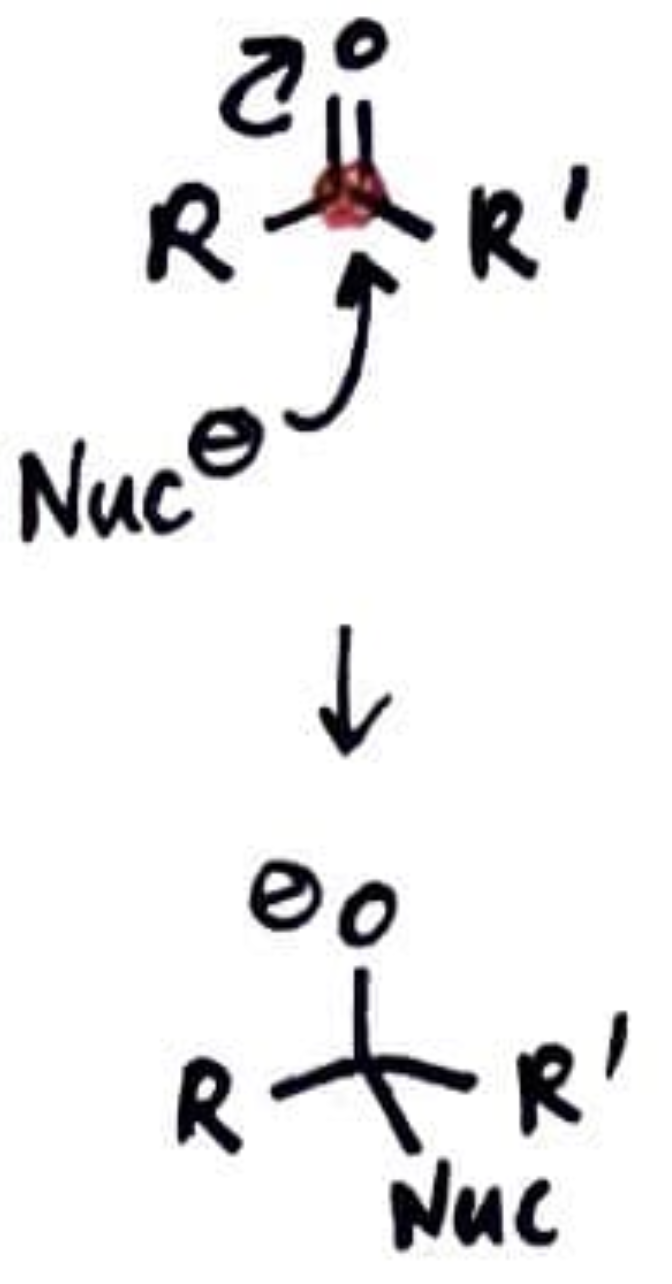
\includegraphics[width=0.23\linewidth]{carbonylRxna.png}
            \caption{As electrophile.}
            \label{fig:carbonylRxna}
        \end{subfigure}
        \begin{subfigure}[b]{0.4\linewidth}
            \centering
            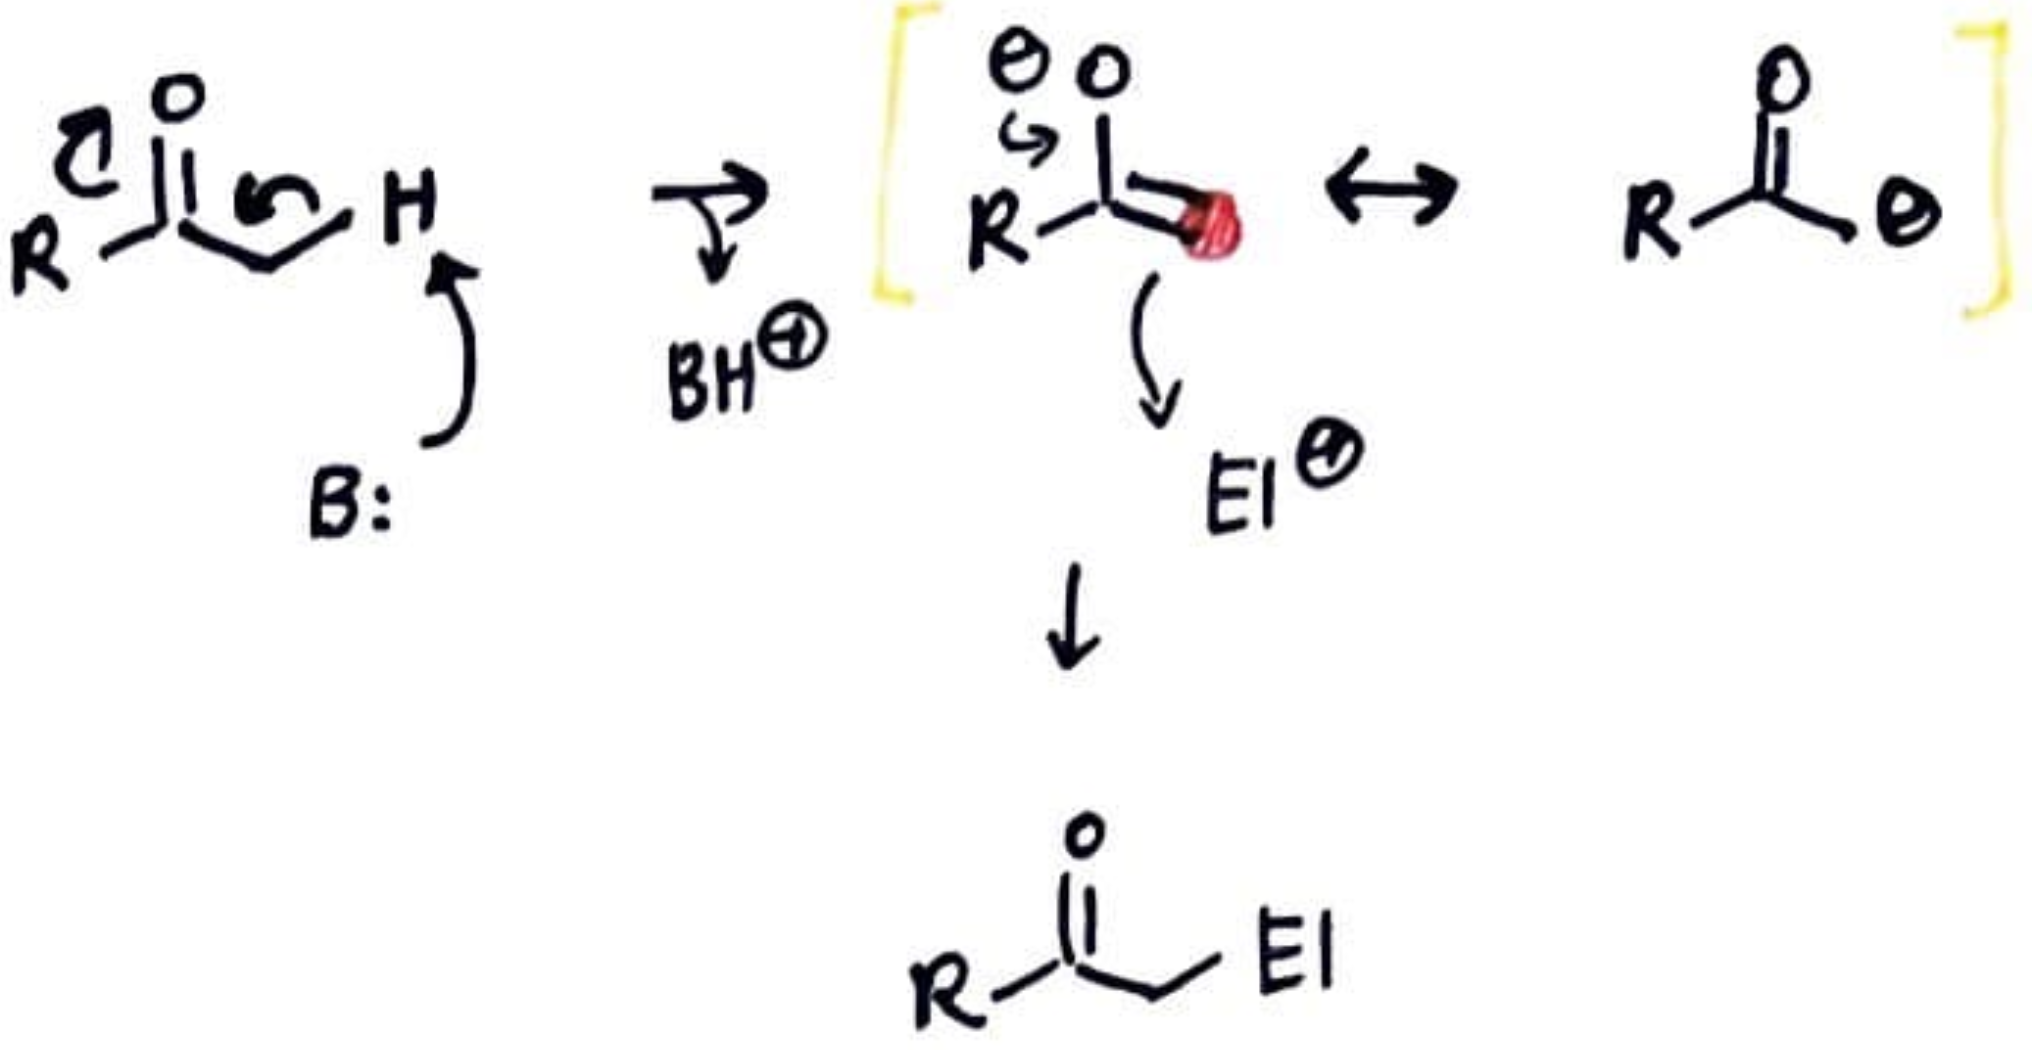
\includegraphics[width=0.9\linewidth]{carbonylRxnb.png}
            \caption{As nucleophile.}
            \label{fig:carbonylRxnb}
        \end{subfigure}
        \caption{Carbonyl-based chemical reactions.}
        \label{fig:carbonylRxn}
    \end{figure}
    \begin{itemize}
        \item Carbonyls have two important modes of reactivity.
        \item We've already discussed how carbonyls can act as electrophiles (Figure \ref{fig:carbonylRxna}).
        \begin{itemize}
            \item This yields a tetrahedral intermediate, as we've discussed.
        \end{itemize}
        \item The other mode of reactivity --- which is new and our focus --- is that we can deprotonate at the $\alpha$-carbon to make a nucleophilic species (Figure \ref{fig:carbonylRxnb}).
        \begin{itemize}
            \item The major resonance structure will be the oxygen-centered one (because oxygen is more electronegative).
            \item However, most reactions we're interested in proceed at carbon.
        \end{itemize}
    \end{itemize}
    \item Key concept: Oxygen \emph{enables} this mode of reactivity stabilizing the negative charge.
    \begin{figure}[h!]
        \centering
        \begin{subfigure}[b]{0.25\linewidth}
            \centering
            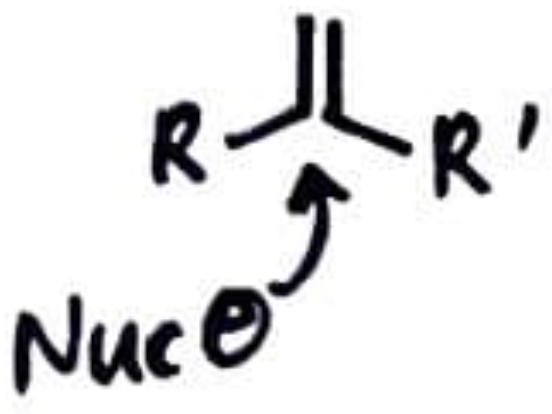
\includegraphics[width=0.38\linewidth]{alkeneCarbonyla.png}
            \caption{Not as electrophiles.}
            \label{fig:alkeneCarbonyla}
        \end{subfigure}
        \begin{subfigure}[b]{0.25\linewidth}
            \centering
            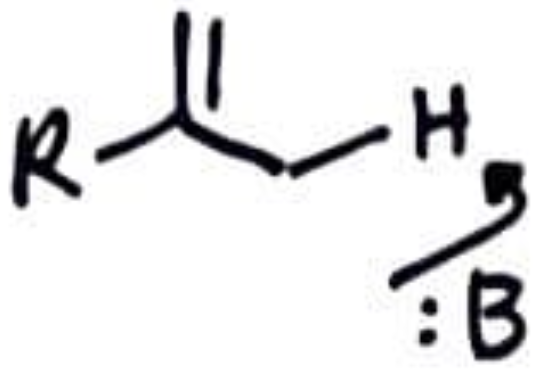
\includegraphics[width=0.38\linewidth]{alkeneCarbonylb.png}
            \caption{Not as nucleophiles.}
            \label{fig:alkeneCarbonylb}
        \end{subfigure}
        \caption{Alkenes do not react via carbonyl-analogous pathways.}
        \label{fig:alkeneCarbonyl}
    \end{figure}
    \begin{itemize}
        \item For the purposes of 5.13, analogous addition to alkenes (Figure \ref{fig:alkeneCarbonyla}) and $\alpha$-deprotonation of alkenes (Figure \ref{fig:alkeneCarbonylb}) is very rare.
    \end{itemize}
    \item Let's now discuss tautomers.
    \begin{figure}[h!]
        \centering
        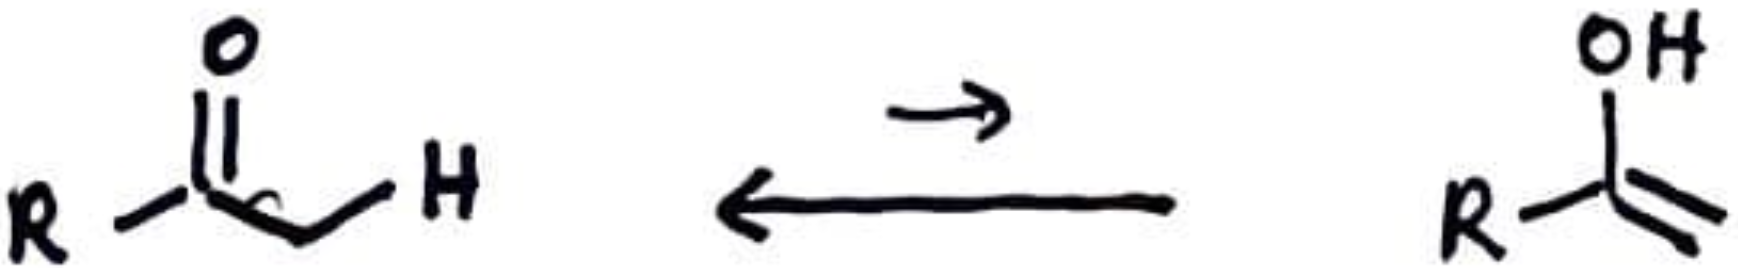
\includegraphics[width=0.32\linewidth]{ketoEnol.png}
        \caption{Keto-enol tautomerization.}
        \label{fig:ketoEnol}
    \end{figure}
    \begin{itemize}
        \item Ketones can tautomerize to \textbf{enols} (a portmanteau of alk\underline{en}e and alcoh\underline{ol}).
        \item The keto and enol form are known as \textbf{tautomers}.
        \item The equilibrium favors the keto form by far (about a million to one; we'll only have $0.001\%$ enol).
    \end{itemize}
    \item Catalysts can speed up the inverconversion, but they can't change the equilibrium.
    \begin{itemize}
        \item Let's discuss the mechanism by which bases and acids speed this process up, though.
    \end{itemize}
    \pagebreak
    \item Base-catalyzed keto-enol tautomerization mechanism.
    \begin{figure}[h!]
        \centering
        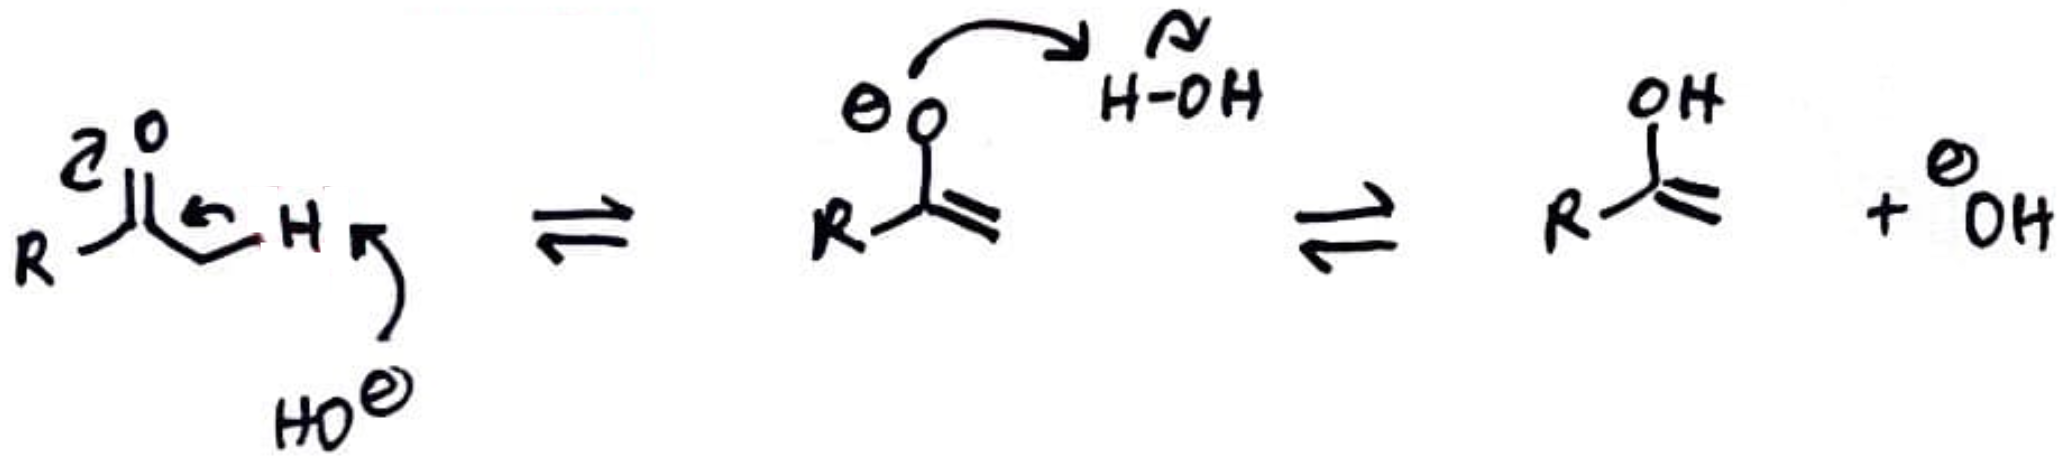
\includegraphics[width=0.55\linewidth]{ketoEnolBase.png}
        \caption{Keto-enol tautomerization mechanism (base-catalyzed).}
        \label{fig:ketoEnolBase}
    \end{figure}
    \begin{itemize}
        \item The $\alpha$-carbon of a ketone has $\pKa\approx 20$.
        \begin{itemize}
            \item This is a good number to memorize, not because you'll ever be tested on it but because understanding relative $\pKa$'s will aid your chemical intuition.
        \end{itemize}
        \item Hydroxide can speed up this process by deprotonating the $\alpha$-carbon.
        \begin{itemize}
            \item Then we just protonate the oxygen.
        \end{itemize}
        \item Recall that we still have $\Keq\ll 1$.
    \end{itemize}
    \item Acid-catalyzed keto-enol tautomerization mechanism.
    \begin{figure}[h!]
        \centering
        \begin{subfigure}[b]{\linewidth}
            \centering
            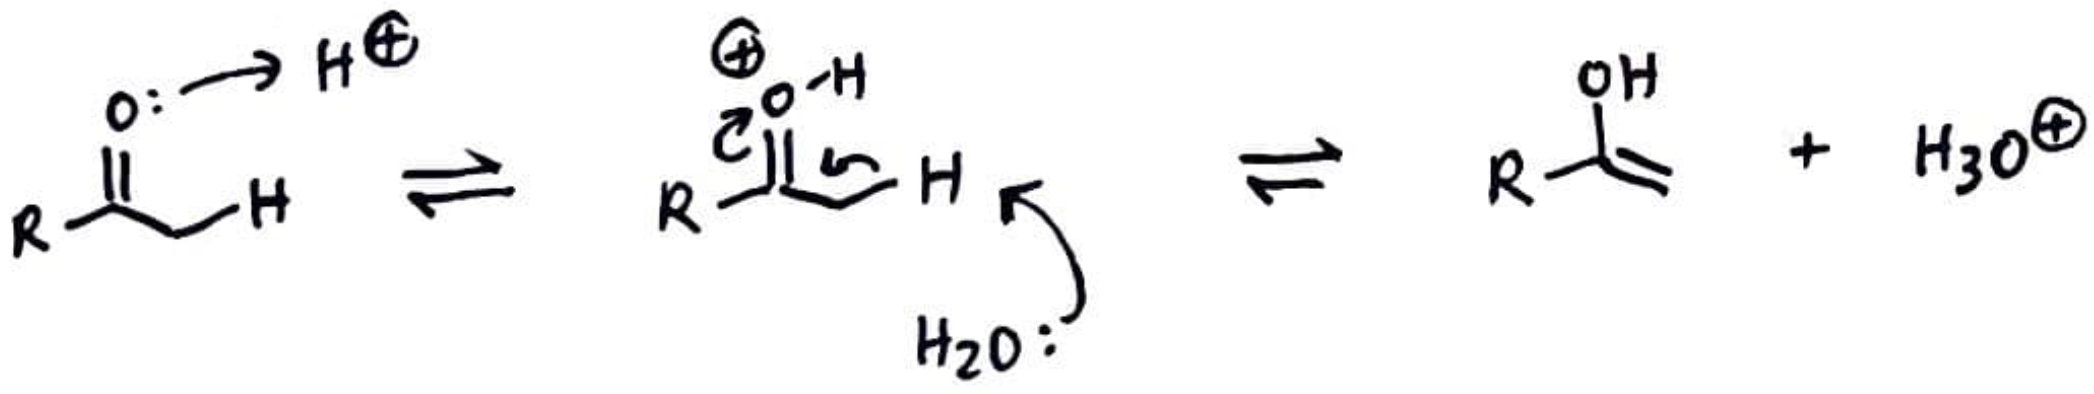
\includegraphics[width=0.62\linewidth]{ketoEnolAcida.png}
            \caption{Correct mechanism.}
            \label{fig:ketoEnolAcida}
        \end{subfigure}\\[2em]
        \begin{subfigure}[b]{\linewidth}
            \centering
            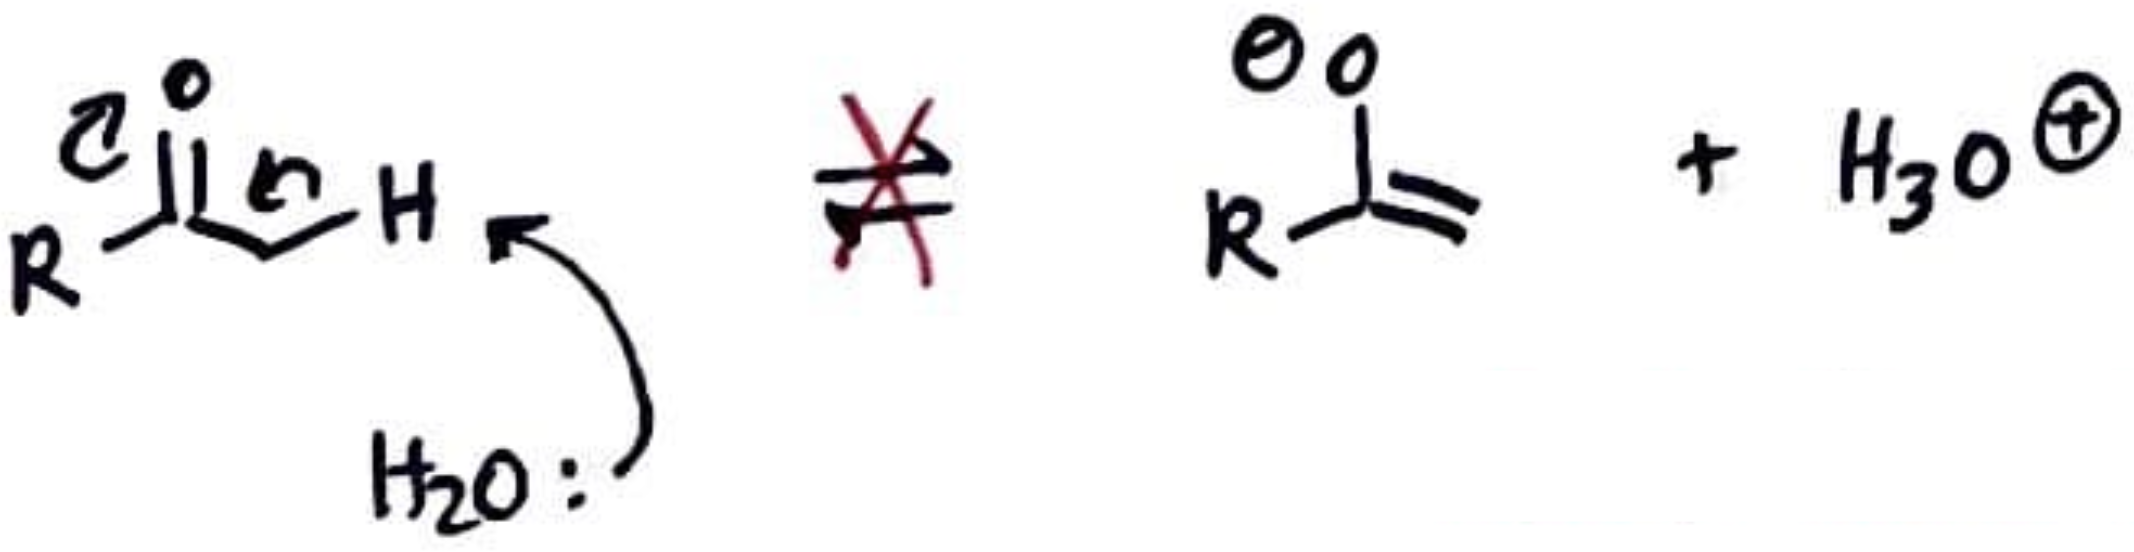
\includegraphics[width=0.4\linewidth]{ketoEnolAcidb.png}
            \caption{Incorrect mechanism.}
            \label{fig:ketoEnolAcidb}
        \end{subfigure}
        \caption{Keto-enol tautomerization mechanism (acid-catalyzed).}
        \label{fig:ketoEnolAcid}
    \end{figure}
    \begin{itemize}
        \item We can either write the reagents equivalently as \ce{H+}/\ce{H2O} or \ce{H3O+}.
        \item As we've been doing, we begin by protonating the carbonyl.
        \item Then the best base in solution comes and deprotonates the $\alpha$-carbon.
        \begin{itemize}
            \item Water isn't a great base, but it's all we've got.
        \end{itemize}
        \item Note that we do \emph{not} do deprotonation first and protonation second, as drawn in Figure ??b.
        \begin{itemize}
            \item Remember that anions cannot exist in acidic solution!
        \end{itemize}
    \end{itemize}
    \item So this is all great, but what if we don't believe Prof. Buchwald that tautomerization occurs?
    \begin{itemize}
        \item It's good to question things in science!
        \item Many times, we've assumed things that later experiments have proven incorrect.
    \end{itemize}
    \pagebreak
    \item We can find evidence for enolization via an isotopic labeling study.
    \begin{figure}[h!]
        \centering
        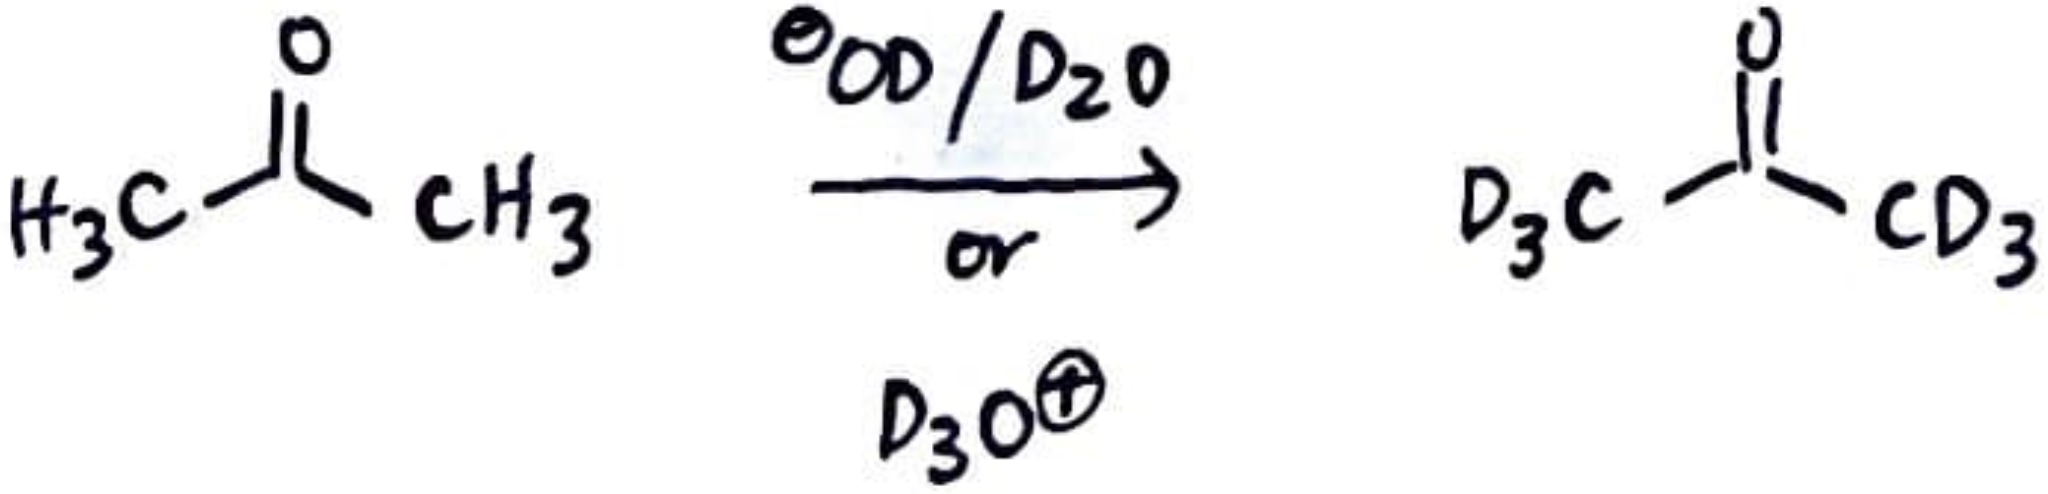
\includegraphics[width=0.4\linewidth]{ketoEnolIsotope.png}
        \caption{Isotopic labeling provides evidence for keto-enol tautomerization.}
        \label{fig:ketoEnolIsotope}
    \end{figure}
    \begin{itemize}
        \item If we dissolve acetone in basic deuterated water and deuteroxide (or acid), we will eventually obtain deuteroacetone.
        \item The mechanism proceeds analogously to Figure \ref{fig:ketoEnolBase} or \ref{fig:ketoEnolAcida}, except that our reagents are all \ce{DO-} and \ce{D2O}.
        \begin{itemize}
            \item In particular, we replace each of the six hydrogens one at a time with deuterium, eventually leading to the product.
            \item We form the fully deuterated product instead of a \ce{H}/\ce{D}-mixed product because we assume that the concentration of deuterated acid or base and water is \emph{much} greater than the concentration of acetone. This is similar to the swamping effect in Figure \ref{fig:transesterEqa}.
        \end{itemize}
    \end{itemize}
    \item We now move onto Topic B: $\alpha$-halogenation of ketones.
    \begin{itemize}
        \item We can do this with chlorine, bromine, or iodine.
    \end{itemize}
    \item Base-promoted $\alpha$-halogenation mechanism.
    \begin{figure}[h!]
        \centering
        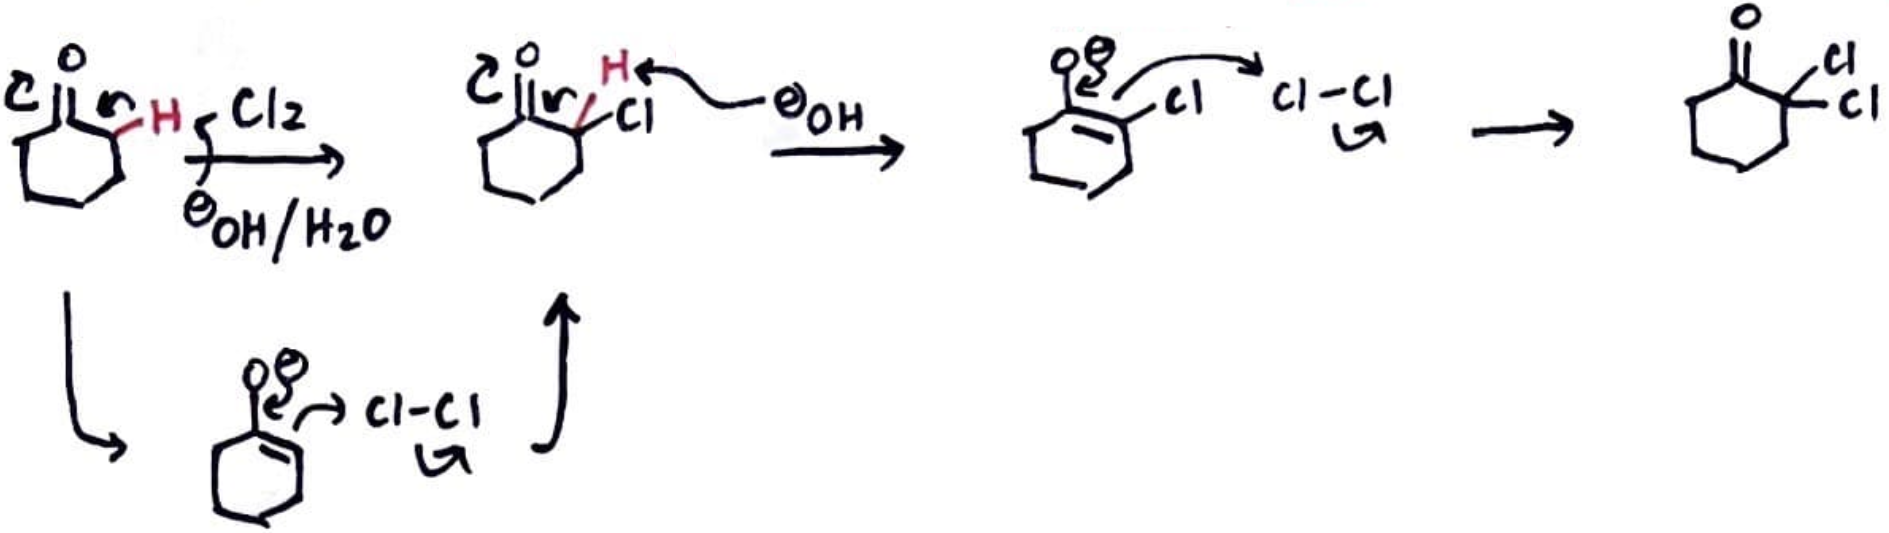
\includegraphics[width=0.8\linewidth]{alphaHaloBase.png}
        \caption{$\alpha$-halogenation mechanism (base-promoted).}
        \label{fig:alphaHaloBase}
    \end{figure}
    \begin{itemize}
        \item Imagine we mix cyclohexanone with chlorine gas under basic conditions. What's going to happen?
        \item We'll form a small amount of enolate, and then chlorinate to form $\alpha$-chlorocyclohexanone.
        \begin{itemize}
            \item We declare victory!
            \item Except that the world is a harsh place and --- like in Figure \ref{fig:redAmin12a} --- we can get further reactivity.
        \end{itemize}
        \item In particular, the hydrogen geminal to the $\alpha$-chlorine is now \emph{more} acidic (proximity to an EWG, so anion is stabilized).
        \begin{itemize}
            \item Thus, we can react again to get $\alpha$-dichlorocyclohexanone.
        \end{itemize}
        \item Thus, this reaction is not good\dots except in one case.
    \end{itemize}
    \pagebreak
    \item The iodoform reaction.
    \begin{figure}[h!]
        \centering
        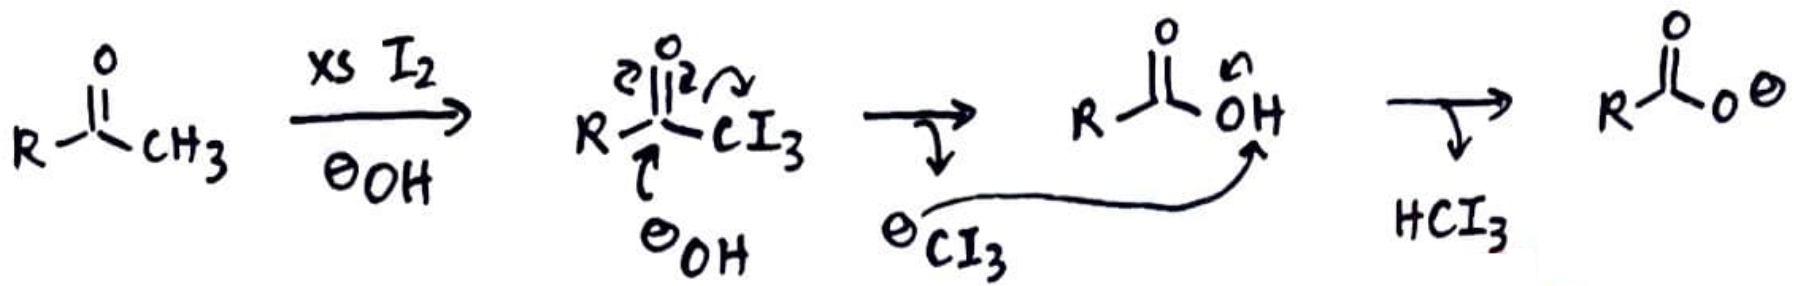
\includegraphics[width=0.7\linewidth]{iodoform.png}
        \caption{Iodoform reaction.}
        \label{fig:iodoform}
    \end{figure}
    \begin{itemize}
        \item In the first step, we have three successive iodinations to yield the triiodomethylketone.
        \item This is such a strong EWG and good leaving group that the triiodomethylketone acts kind of like an acid chloride.
        \begin{itemize}
            \item In particular, we get an addition-elimination mechanism that kicks out the triiodomethanide anion.
            \item This anion can then be protonated by the resultant carboxylic acid to yield iodoform (\ce{HCI3}) and a stable carboxylate.
        \end{itemize}
        \item Iodoform precipitates as a yellow solid.
        \begin{itemize}
            \item In the olden days, it used to be a test for a ketone.
            \item Before we had NMR, mass spec, and other kinds of spectroscopy, we had a bunch of test reagents that we would add to our compounds to determine what it was.
            \item Essentially, if we had a compound and we didn't know what it was but thought it was a ketone, we could confirm or deny this by adding iodine and base to our mixture!
        \end{itemize}
    \end{itemize}
    \item What does it mean when Prof. Buchwald draws a circular arrow from a carbonyl $\pi$-bond back to it?
    \begin{itemize}
        \item They use this in \textcite{bib:Clayden}!
        \item This is a shorthand for the two-step addition-elimination process, in which electrons kick up in a first step and then kick back down in a second step.
        \item This is similar to how we shorthand a two-step proton transfer as "PT!"
    \end{itemize}
    \item So how do we make mono-$\alpha$-haloketones, if that's our goal?
    \begin{itemize}
        \item Use acid-catalyzed $\alpha$-halogenation!
    \end{itemize}
    \item Acid-catalyzed $\alpha$-halogenation mechanism.
    \begin{figure}[h!]
        \centering
        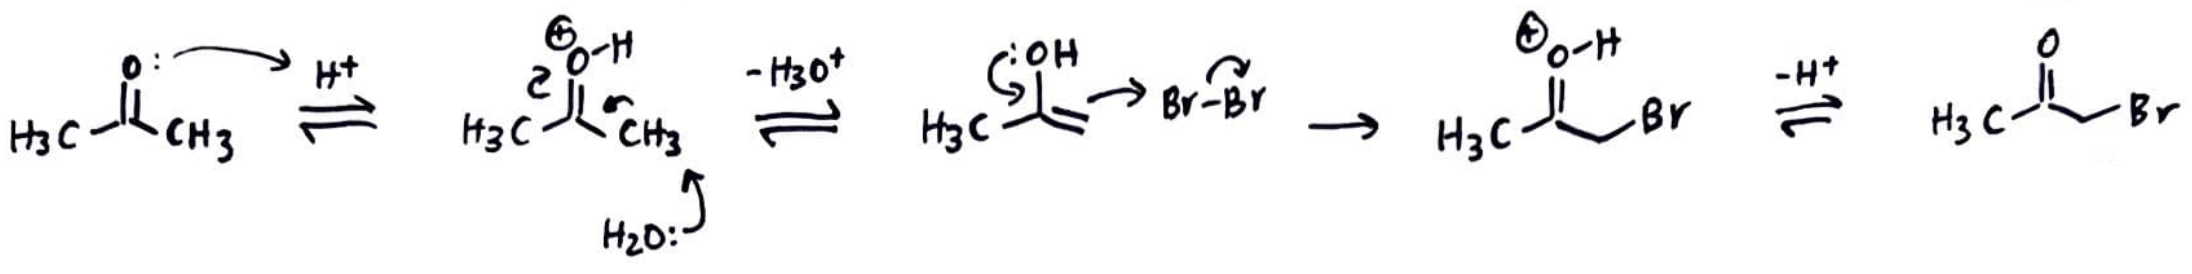
\includegraphics[width=\linewidth]{alphaHaloAcid.png}
        \caption{$\alpha$-halogenation mechanism (acid-catalyzed).}
        \label{fig:alphaHaloAcid}
    \end{figure}
    \begin{itemize}
        \item Acids encourage the rate of formation of the enol.
        \item Then if we do this in the presence of bromine, we'll get $\alpha$-bromoacetone (following deprotonation).
        \item Now the product is \emph{less} reactive than the starting material (because the bromine EWG stabilizes the carbonyl and disfavors protonation of it).
        \item Takeaway: Acid-catalyzed $\alpha$-halogenation is selective for monohalogenation.
        \item This process is used to synthesize a lot of medicines and drug molecules.
    \end{itemize}
    \pagebreak
    \item We now move onto Topic C: $\alpha$-alkylation.
    \begin{itemize}
        \item This is the heavy hitter; a really, really important reaction of ketones.
    \end{itemize}
    \item General form.
    \begin{figure}[h!]
        \centering
        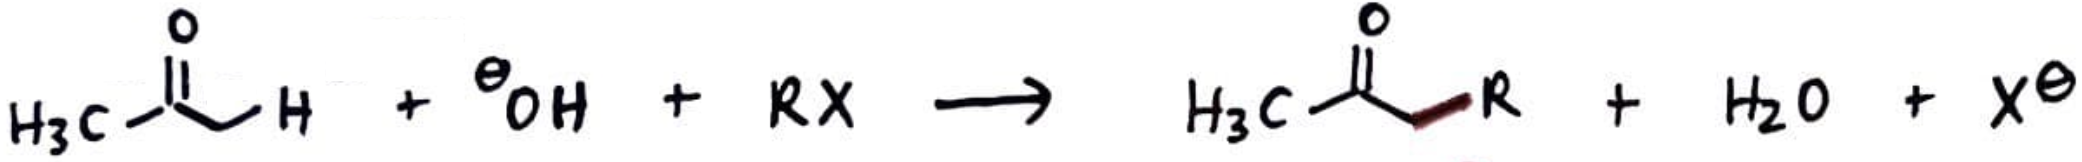
\includegraphics[width=0.65\linewidth]{alphaAlk.png}
        \caption{$\alpha$-alkylation.}
        \label{fig:alphaAlk}
    \end{figure}
    \begin{itemize}
        \item Suppose we want to convert a ketone into a new compound where we've formed a \ce{C-C} bond.
        \item The other reagent is a primary or secondary alkyl halide.
    \end{itemize}
    \item Drawing a mechanism for this doesn't seem too bad at first.
    \begin{itemize}
        \item We may deprotonate to the enolate and attack the alkyl halide to start.
        \item But there is a complication.
        \begin{itemize}
            \item We get lots of side reactions!
        \end{itemize}
        \item In 5.13, we're all about efficiency and elegance, so this is not good.
    \end{itemize}
    \item There are several solutions to this issue, which we'll discuss presently.
    \item Solution 1: Use lithium diisopropylamide (LDA).
    \begin{figure}[h!]
        \centering
        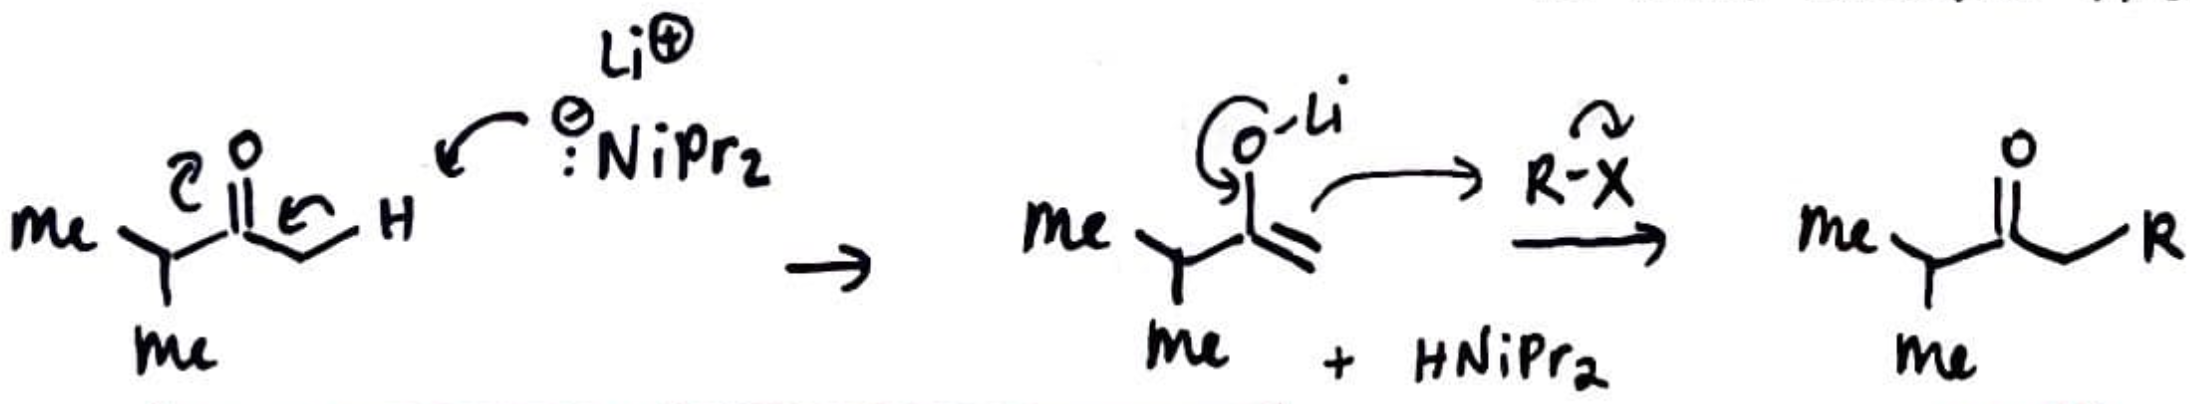
\includegraphics[width=0.6\linewidth]{alphaAlkLDA.png}
        \caption{$\alpha$-alkylation with lithium diisopropylamide.}
        \label{fig:alphaAlkLDA}
    \end{figure}
    \begin{itemize}
        \item See Figure \ref{fig:amineEx2b} for the structure and synthesis of LDA.
        \item Helpful characteristics of LDA.
        \begin{itemize}
            \item LDA is a strong base.
            \item It is secondary and hence hindered (therefore a poor nucleophile).
            \item The conjugate acid of LDA has $\pKa\approx 35$.
            \item Thus, it will only deprotonate and not do any competitive addition chemistry!
        \end{itemize}
        \item We begin with an essentially irreversible deprotonation to the enolate.
        \item This is followed by 100\% conversion to the alkylated product.
    \end{itemize}
    \item Using LDA is a relatively modern solution --- only about 50 years old.
    \begin{itemize}
        \item However, organic chemistry has been around for close to 250 years!
        \item The roots of organic chemistry are in the old German dye industry, which morphed into the present-day pharmaceutical industry.
        \item So how did people do this stuff before LDA? Via solution 2.
    \end{itemize}
    \pagebreak
    \item Solution 2: Malonate ester synthesis.
    \begin{figure}[h!]
        \centering
        \begin{subfigure}[b]{\linewidth}
            \centering
            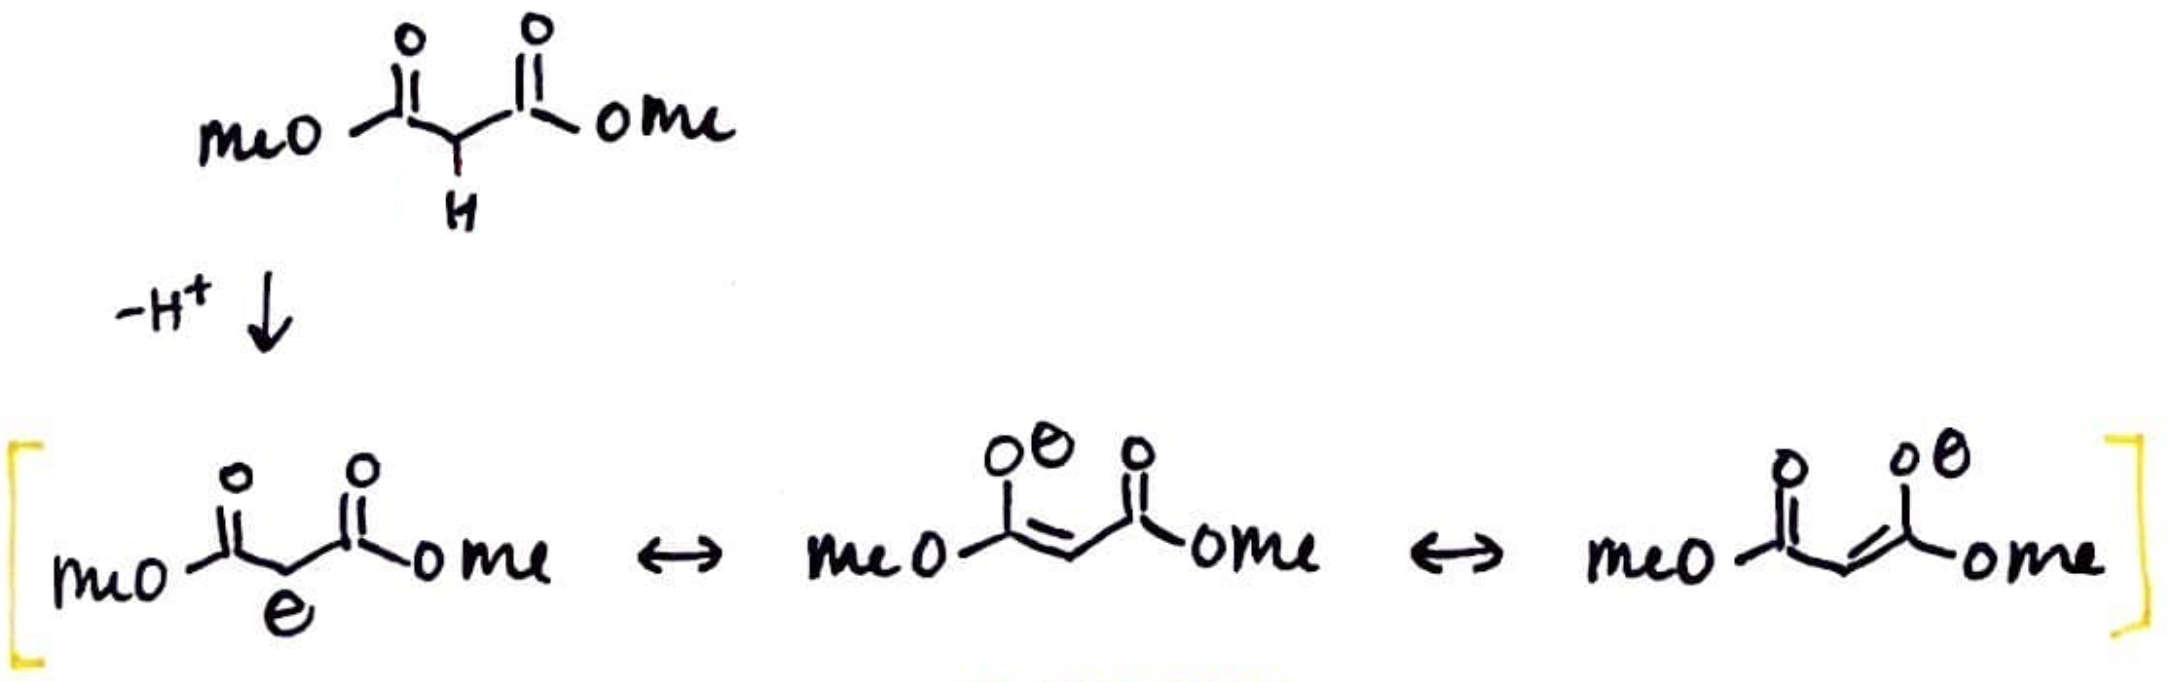
\includegraphics[width=0.6\linewidth]{alphaAlkMalEstera.png}
            \caption{Malonate ester resonance.}
            \label{fig:alphaAlkMalEstera}
        \end{subfigure}\\[2em]
        \begin{subfigure}[b]{\linewidth}
            \centering
            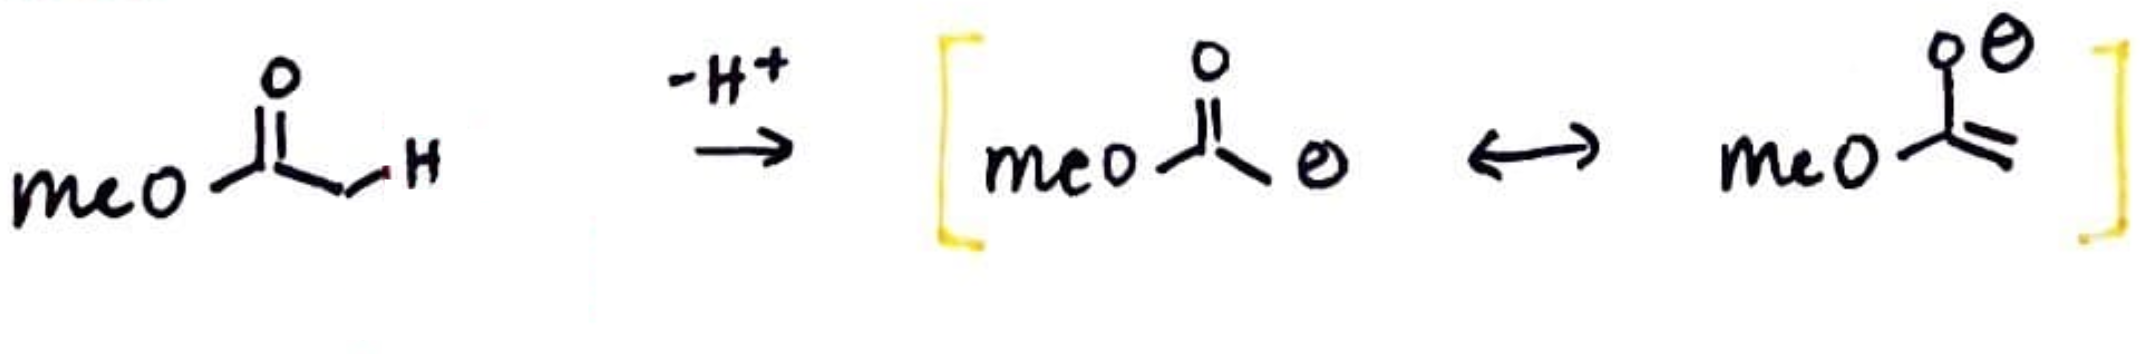
\includegraphics[width=0.5\linewidth]{alphaAlkMalEsterb.png}
            \caption{Regular ester resonance.}
            \label{fig:alphaAlkMalEsterb}
        \end{subfigure}
        \caption{$\alpha$-alkylation with malonate esters.}
        \label{fig:alphaAlkMalEster}
    \end{figure}
    \begin{itemize}
        \item The starting material has esters on both sides (either ethyl or methyl; it doesn't matter).
        \item The important thing is that for the malonate ester, $\pKa\approx 13$.
        \begin{itemize}
            \item In contrast, a regular ester has $\pKa\approx 25$.
        \end{itemize}
        \item Why this drastic difference in $\pKa$?
        \begin{itemize}
            \item The deprotonated malonate ester's anion has more resonance forms (two adjacent carbonyls into which to delocalze!) than the deprotonated ester (only one adjacent carbonyl).
        \end{itemize}
        \item This difference leads us to call the deprotonated malonate ester a \textbf{soft enolate}.
        \begin{itemize}
            \item These characteristics make it very easy and safe to work with, so it's often used at scale.
        \end{itemize}
    \end{itemize}
    \item We'll now quickly introduce a topic that we'll also discuss more next time.
    \item Kinetic vs. thermodynamic enolates.
    \item \textbf{Kinetic} (enolate): The enolate generated by deprotonation at the less-substituted position, all else being equal.
    \item Example: LDA (really big and bulky) will selectively form the kinetic enolate at the unsubstituted position of $\alpha$-methylcyclohexanone.
    \begin{figure}[h!]
        \centering
        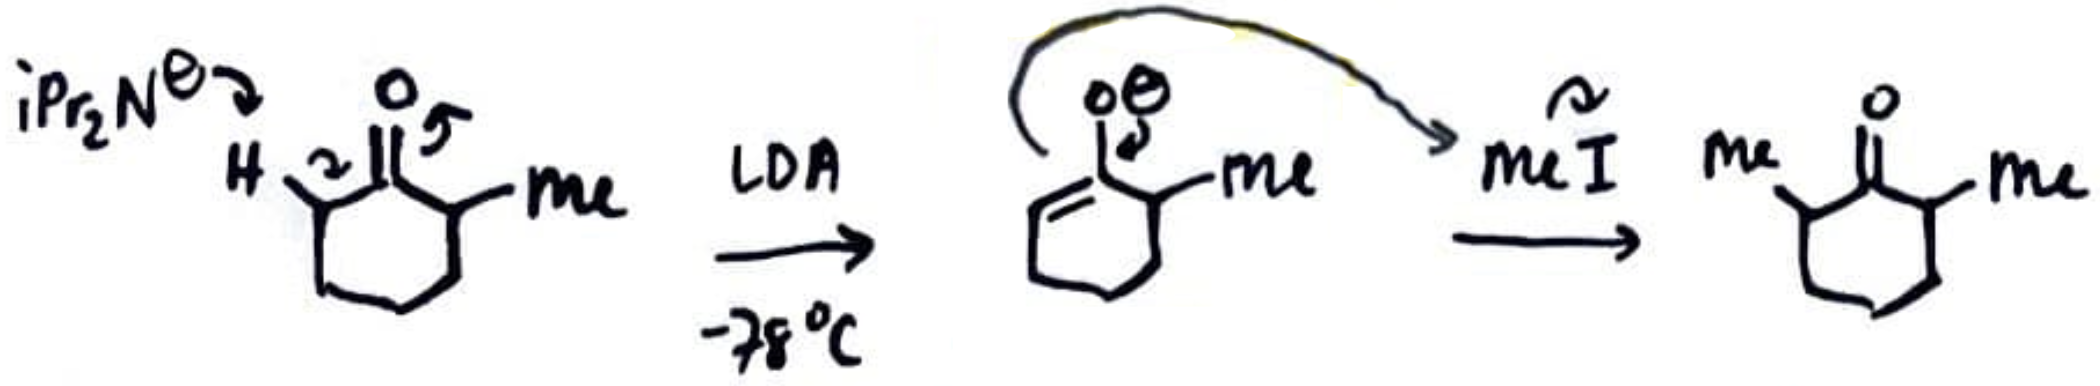
\includegraphics[width=0.6\linewidth]{enolateKinetic.png}
        \caption{Kinetic enolate formation.}
        \label{fig:enolateKinetic}
    \end{figure}
    \begin{itemize}
        \item This enolate could then be used --- for example --- to attack methyl iodide (\ce{MeI}) and alkylate.
        \item Note that this process would most likely form a mixture of stereoisomers.
    \end{itemize}
    \pagebreak
    \item \textbf{Thermodynamic} (enolate): The enolate that is more stable.
    \item Example: Potassium \emph{t}-butoxide (\ce{KO{}^{\emph{t}}Bu}) has $\pKa\approx\text{\numrange{16}{18}}$, so it deprotonates $\alpha$-methylcyclohexanone reversibly until we get the more stable one.
    \begin{figure}[h!]
        \centering
        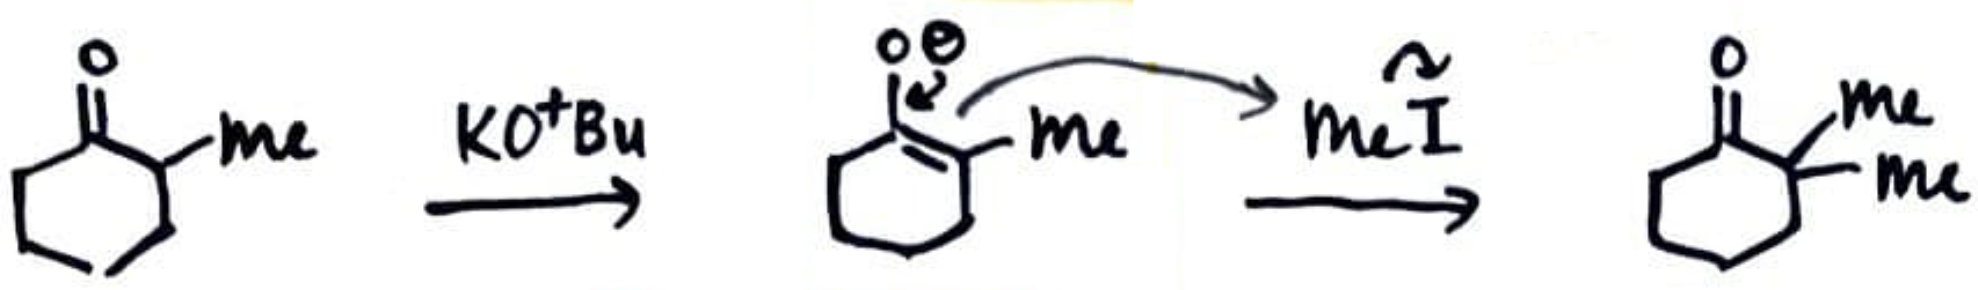
\includegraphics[width=0.55\linewidth]{enolateThermodynamic.png}
        \caption{Thermodynamic enolate formation.}
        \label{fig:enolateThermodynamic}
    \end{figure}
    \begin{itemize}
        \item Treating this with \ce{MeI} then generates the $\alpha$-dimethylated form of cyclohexanone.
    \end{itemize}
    \item You can add in \ce{Me3SiCl} to trap enolates the silyl enol ether.
    \begin{figure}[h!]
        \centering
        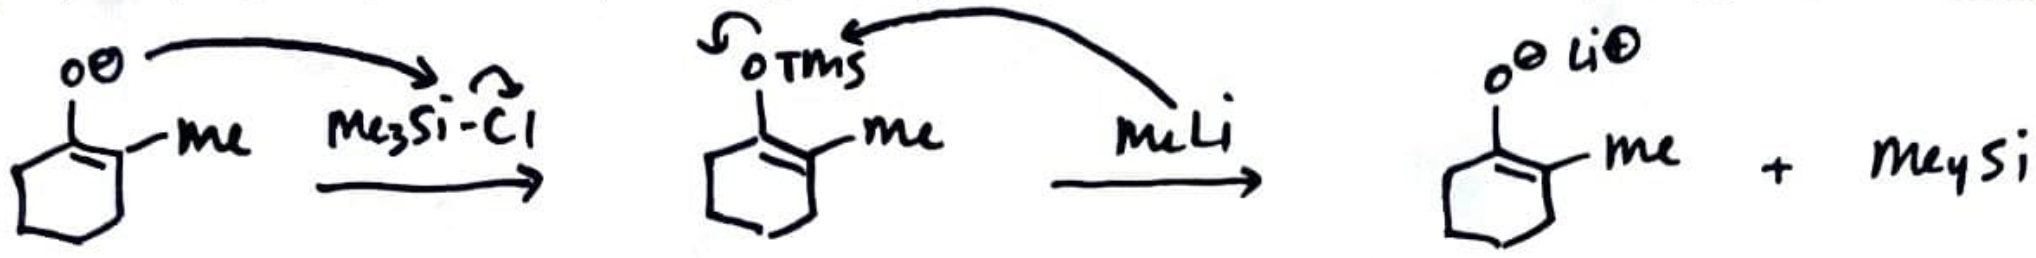
\includegraphics[width=0.75\linewidth]{enolateTMS.png}
        \caption{Trapping enolates as silyl enol ethers.}
        \label{fig:enolateTMS}
    \end{figure}
    \begin{itemize}
        \item This silyl protecting group could then be removed with \ce{MeLi}, regenerating the enolate and yielding tetramethylsilane (\ce{SiMe4}) as a byproduct.
        \item In the deprotection step, the methyl anion attacks the silicon atom in the TMS group, engaging in an S\textsubscript{N}2 displacement.
    \end{itemize}
\end{itemize}



\section{Enolate Alkylation}
\begin{itemize}
    \item \marginnote{11/18:}We will not begin with a line-by-line review of last lecture; rather, we will clarify some things.
    \item Lecture 29 recap.
    \begin{itemize}
        \item Recall kinetic vs. thermodynamic enolates (Figures \ref{fig:enolateKinetic} \& \ref{fig:enolateThermodynamic}).
        \item When we use a strong, hindered base (like \ce{LDA}), we abstract the unhindered proton to form the kinetic enolate.
        \begin{itemize}
            \item This process is irreversible, and yields 100\% of the kinetic enolate.
            \item The process is irreversible because $\pKa\approx 35$ for the conjugate acid of LDA (lithium diisopropylamine), so this conjugate acid cannot react backwards.
        \end{itemize}
        \item Use of a somewhat strong, somewhat bulky base (like \ce{KO{}^{\emph{t}}Bu} in \ce{{}^{\emph{t}}BuOH}).
        \begin{itemize}
            \item This process is highly reversible, so we'll abstract the unhindered proton first. But then the enolate can react backwards with \ce{{}^{\emph{t}}BuOH} to reform the ketone!
            \item This process is highly reversible because $\pKa\approx 19$ for \ce{{}^{\emph{t}}BuOH}, so this conjugate acid \emph{can} react backwards.
            \item However, when we eventually deprotonate the hindered proton, we form a more stable enolate that is \emph{less likely} to react backwards.
            \item Thus, the net result is that we form the \emph{thermodynamic} enolate under these conditions.
        \end{itemize}
        \item Both of these enolates can then be trapped with \ce{MeI} into the corresponding $\alpha$-alkylation product.
    \end{itemize}
    \pagebreak
    \item Lecture outline.
    \begin{enumerate}[label={\Alph*.},start=3]
        \item $\alpha$-alkylation.
        \begin{itemize}
            \item Enolate-forming bases.
            \item Enolates from esters (hard to form) and aldehydes (don't form).
            \item Enolate-alkylation electrophiles.
            \item Synthesis of $\alpha$-substituted acetic acid derivatives.
            \item Synthesis of $\alpha$-substituted 1,3-diols.
        \end{itemize}
    \end{enumerate}
    \item We return to Topic C: $\alpha$-alkylation.
    \item Let's consider the properties of several strong bases.
    \begin{table}[h!]
        \centering
        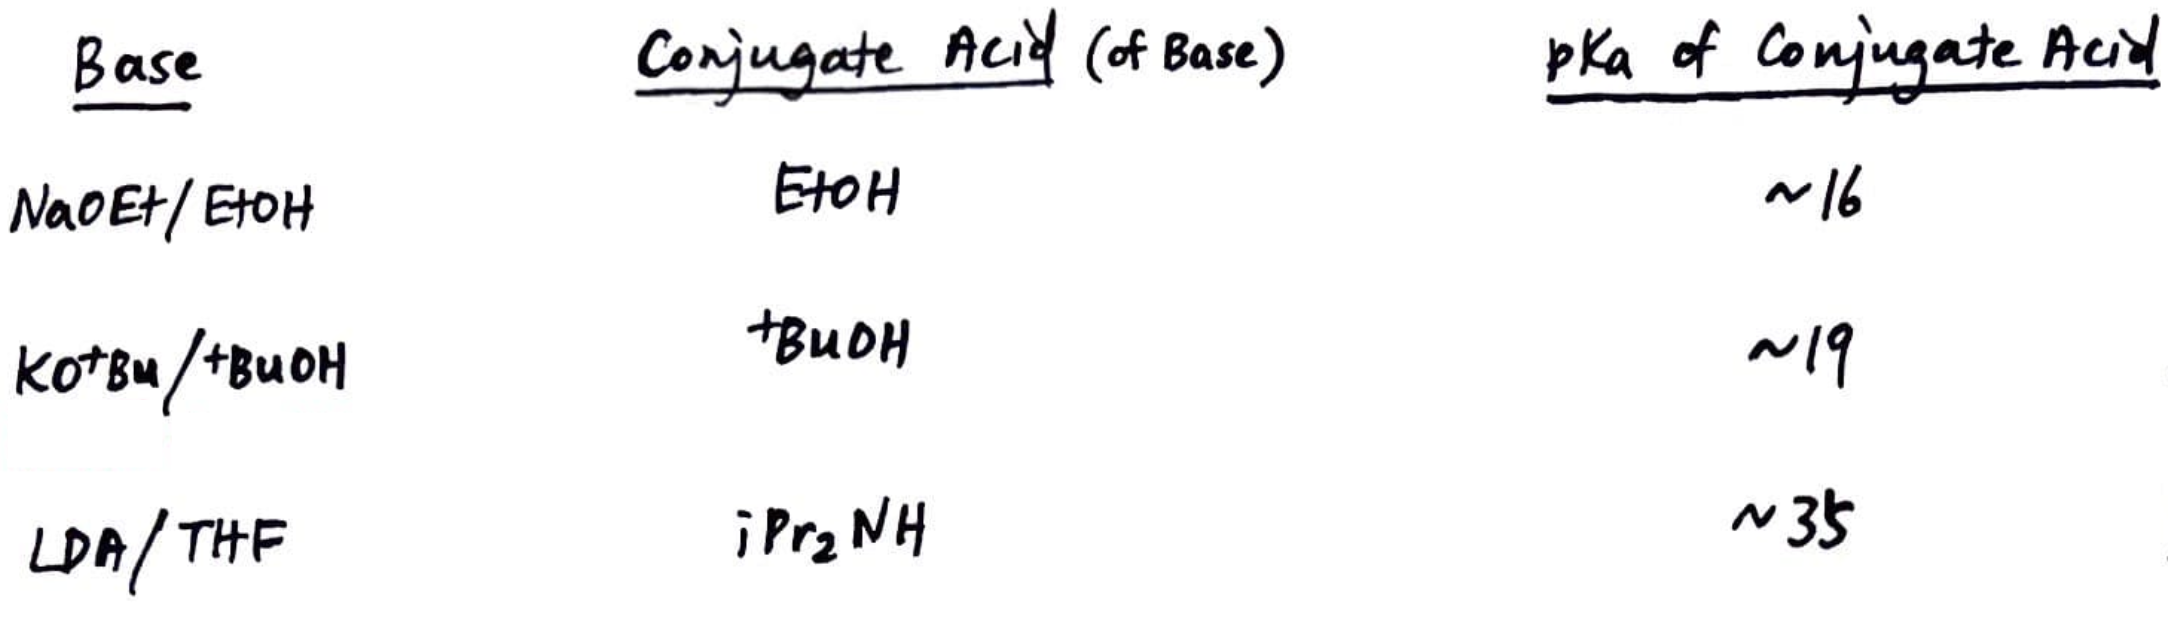
\includegraphics[width=0.6\linewidth]{enolateBase.png}
        \caption{$\pKa$'s of typical enolate-forming bases.}
        \label{tab:enolateBase}
    \end{table}
    \begin{itemize}
        \item The left column shows a base and the solvent in which you use it, not necessarily the base and it's conjugate acid!
        \item It follows from the table that \ce{NaOEt} and \ce{KO{}^{\emph{t}}Bu} are reversible bases, and LDA is an irreversible base.
        \item The difference between the first two is that \ce{KO{}^{\emph{t}}Bu} is bulkier and less nucleophilic.
        \begin{itemize}
            \item So if we're worried about nucleophilic attack as a side reaction, use this!
        \end{itemize}
        \item Otherwise, \ce{NaOEt} is cheaper and more pleasant to work with.
    \end{itemize}
    \item So what happens when we do enolate formation with different bases?
    \begin{itemize}
        \item Suppose that the conjugate acid \ce{B1H} has $\pKa>22$.
        \begin{itemize}
            \item Then the reaction is irreversible.
            \item Example: LDA!
        \end{itemize}
        \item Suppose that the conjugate acid \ce{B2H} has $16<\pKa<22$.
        \begin{itemize}
            \item This reaction is reversible.
            \item Examples: \ce{NaOEt} and \ce{KO{}^{\emph{t}}Bu}!
        \end{itemize}
        \item Suppose that the conjugate acid \ce{B3H} has $\pKa<16$.
        \begin{itemize}
            \item Nothing happens! The base isn't strong enough.
        \end{itemize}
        \item Note: We'll read in \textcite{bib:Clayden} that we can use bases with $\pKa<16$ \emph{if} we pair it with a Lewis acid.
        \begin{itemize}
            \item Example: \underline{T}ri\underline{m}ethyl\underline{s}ilyl chloride (\ce{TMSCl}) and \ce{NEt3}.
        \end{itemize}
        \item Generalizing this.
        \begin{itemize}
            \item Consider the $\pKa$ of our $\alpha$-proton.
            \item If the base is 3 $\pKa$ units weaker or stronger, we get reversible enolate formation.
            \item If the base is more than 3 $\pKa$ units stronger, we get irreversible enolate formation.
            \item If the base is more than 3 $\pKa$ units weaker, no reaction occurs because the base is too weak.
        \end{itemize}
    \end{itemize}
    \item Example: Consider methyl isopropyl ketone.
    \begin{itemize}
        \item Use LDA to deprotonate at the methyl group and form the kinetic enolate.
        \item Use \ce{KO{}^{\emph{t}}Bu} in \ce{{}^{\emph{t}}BuOH} to form the thermodynamic enolate.
    \end{itemize}
    \item How about forming enolates from esters?
    \begin{itemize}
        \item We need LDA because $\pKa\approx 25$ for the ester's $\alpha$-proton.
        \item Indeed, esters have significantly less acidic $\alpha$-protons than ketones.
        \item We also need low temperatures to prevent self-condensation.
    \end{itemize}
    \item How about forming enolates from aldehydes?
    \begin{itemize}
        \item For the purposes of this class, we'll say that aldehyde enolates don't exist.
        \item In reality, aldehyde enolates \emph{do} exist, but they are \emph{so} reactive that even at low temperatures, there is lots of competitive self-condensation.
    \end{itemize}
    \item We now return to alkylations of enolates in more depth.
    \begin{itemize}
        \item There are parallels to S\textsubscript{N}2 reactivity here.
        \item Enolates are more hindered than, for example, cyanide nucleophiles (\ce{CN-}), azide nucleophiles (\ce{N3-}), etc.
        \begin{itemize}
            \item They are also more basic.
        \end{itemize}
        \item For the purposes of 5.13\dots
        \begin{itemize}
            \item We'll say that primary alkyl, methyl, benzyl, and allyl halides react with enolates to do $\alpha$-alkylation.
            \begin{itemize}
                \item The TFs will discuss in recitation why benzyl and allyl halides are "activated!!"
            \end{itemize}
            \item We'll also say that secondary alkyl halides do not react with enolates.
            \begin{itemize}
                \item This is because it's more hindered, so we get more competitive elimination.
            \end{itemize}
        \end{itemize}
        \item Tertiary, vinyl, phenyl, and neopentyl halides \emph{never} react with enolates.
        \begin{itemize}
            \item Note that neopentyl is bad (even though it's primary) because it's \emph{super} bulky.
        \end{itemize}
    \end{itemize}
    \item We now discuss the synthesis of $\alpha$-substituted malonate esters.
    \begin{figure}[h!]
        \centering
        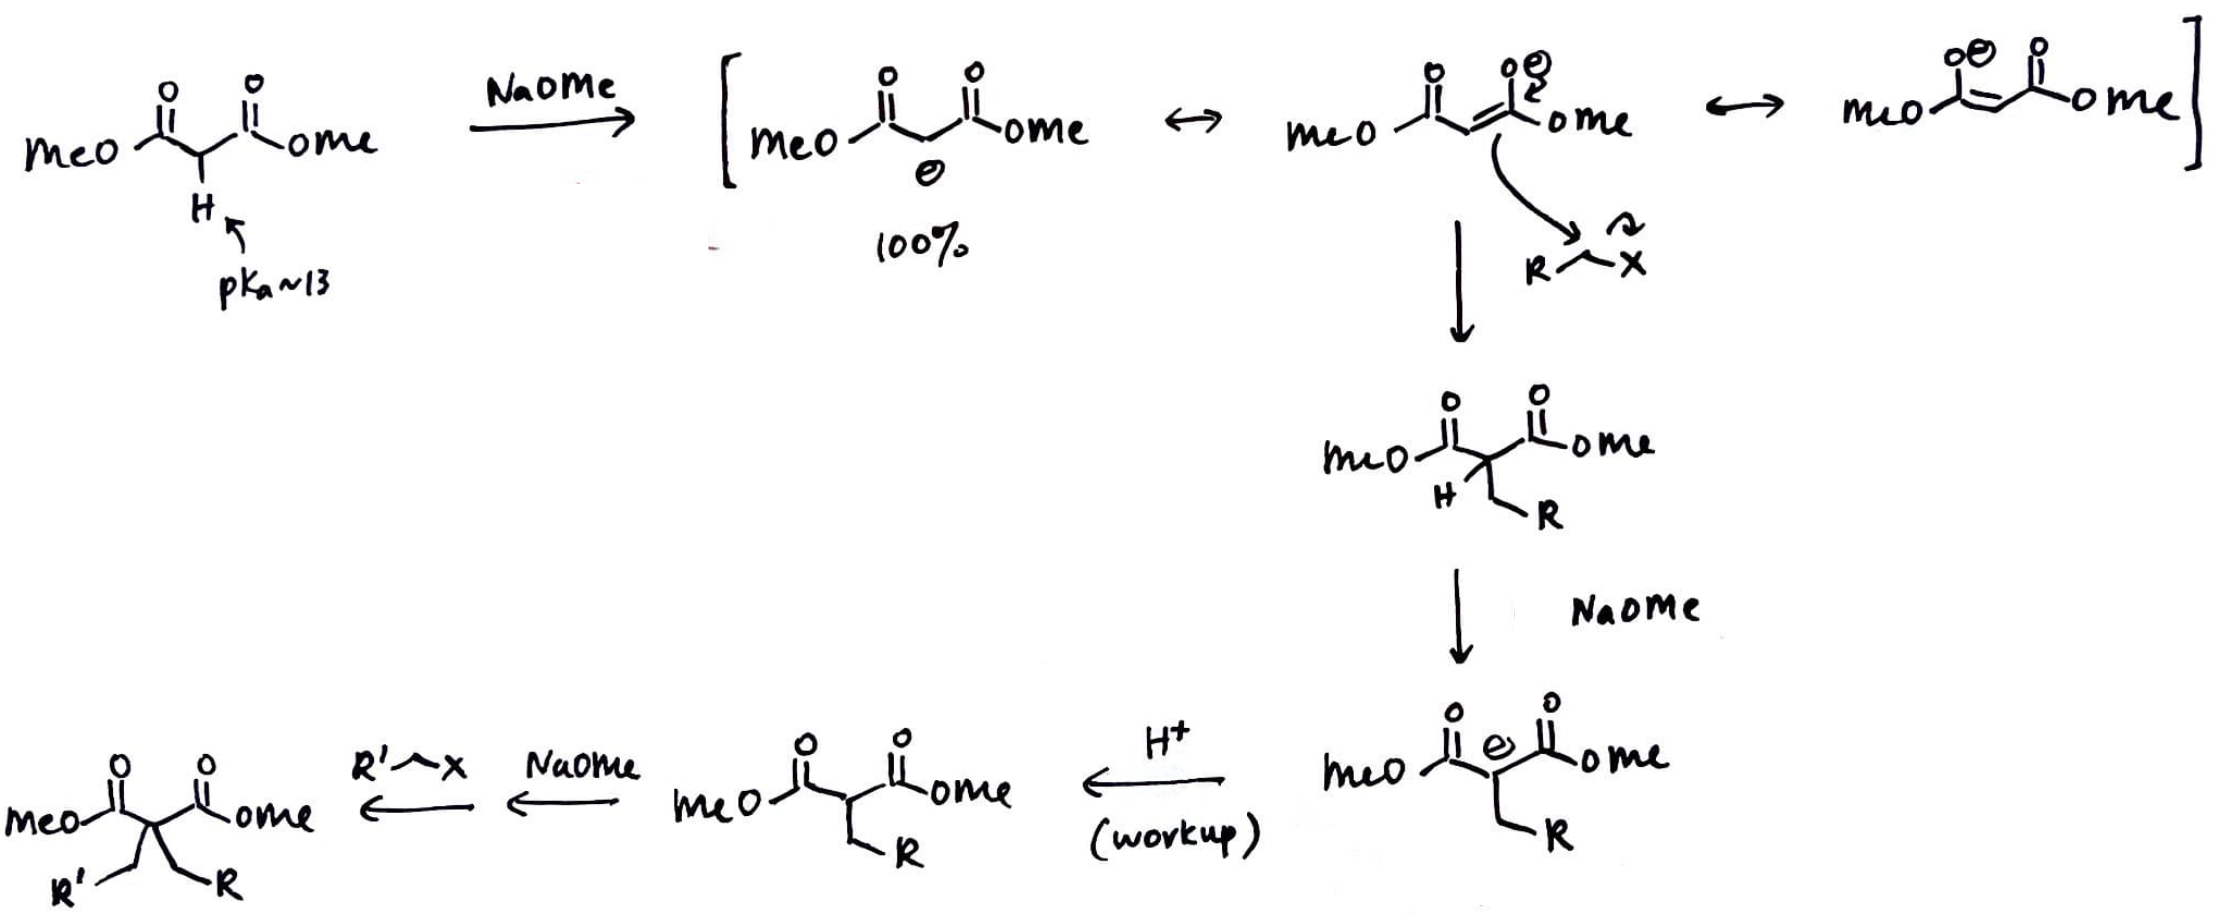
\includegraphics[width=0.9\linewidth]{malEsterSynth.png}
        \caption{Malonate ester synthesis.}
        \label{fig:malEsterSynth}
    \end{figure}
    \pagebreak
    \begin{itemize}
        \item Recall malonate esters from last class (see Figure \ref{fig:alphaAlkMalEstera}).
        \item Since these compounds have $\pKa\approx 13$ at their $\alpha$-protons, \ce{NaOMe} can do 100\% deprotonation.
        \begin{itemize}
            \item Note that we match the base to the ester: Dimethyl malonate should be paired with \ce{NaOMe} in \ce{MeOH} and diethyl malonate should be paired with \ce{NaOEt} in \ce{EtOH}.
            \item This is because we'll have competitive transesterification (see Figure \ref{fig:transesterBase}), so matching the base ensures that we don't get a mixture of products.
        \end{itemize}
        \item Our deprotonated malonate ester can then attack some \ce{C-X} bond, alkylating the $\alpha$-position.
        \item But we're still in basic solution, so our species will be deprotonated until water workup.
        \begin{itemize}
            \item Do assume that we will \emph{not} get competitive dialkylation.
            \item However, alternatively, we could add more base and another \ce{C-X} species to yield a dialkylated species.
        \end{itemize}
        \item These reactions are collectively known as the \textbf{malonate ester synthesis}.
    \end{itemize}
    \item TTQ: Given propane-1,3-diol, \ce{MeI}, and \ce{EtI}, make the product shown in Figure ??a.
    \begin{figure}[h!]
        \centering
        \begin{subfigure}[b]{\linewidth}
            \centering
            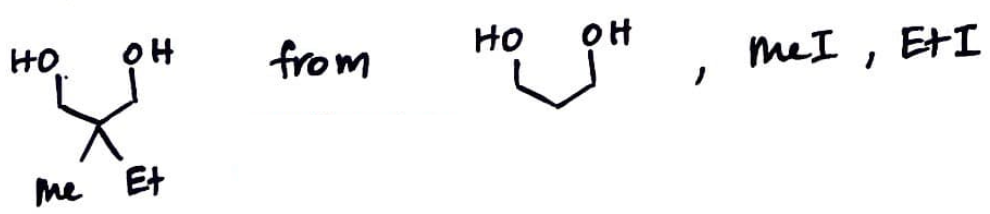
\includegraphics[width=0.4\linewidth]{TTQalpha13diola.png}
            \caption{The desired molecule and starting materials.}
            \label{fig:TTQalpha13diola}
        \end{subfigure}\\[2em]
        \begin{subfigure}[b]{\linewidth}
            \centering
            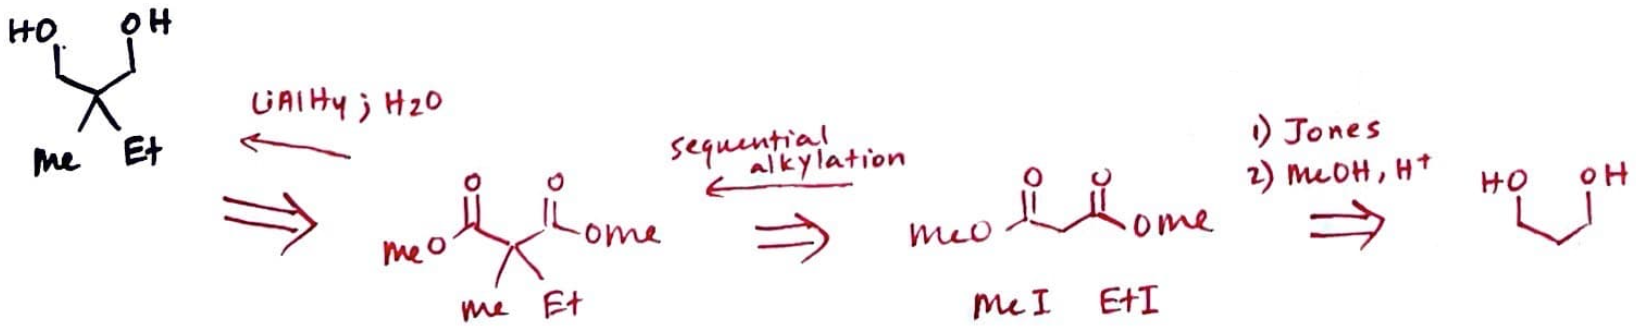
\includegraphics[width=0.65\linewidth]{TTQalpha13diolb.png}
            \caption{Retrosynthetic pathway.}
            \label{fig:TTQalpha13diolb}
        \end{subfigure}
        \caption{TTQ: Synthesis of an $\alpha$-substituted 1,3-diol.}
        \label{fig:TTQalpha13diol}
    \end{figure}
    \begin{itemize}
        \item You might get greedy and start thinking about how to deprotonate the middle carbon directly, but we can't do that; we have to go back to something more reasonable first.
        \item Indeed, we can do a malonate ester synthesis with sequential alkylations followed by LAH reduction to the diol!
        \item Tip: Whenever you see a 1,3-diol, you should ask yourself if a malonate ester can be used!
        \item Note that we make the malonate ester from the 1,3-diol via Jones oxidation (see Figure \ref{fig:OxAlcAlda}) followed by Fischer esterification (see Figure \ref{fig:acylTFischer}).
    \end{itemize}
    \item We now discuss a related process called the \textbf{acetoacetate synthesis}.
    \begin{figure}[h!]
        \centering
        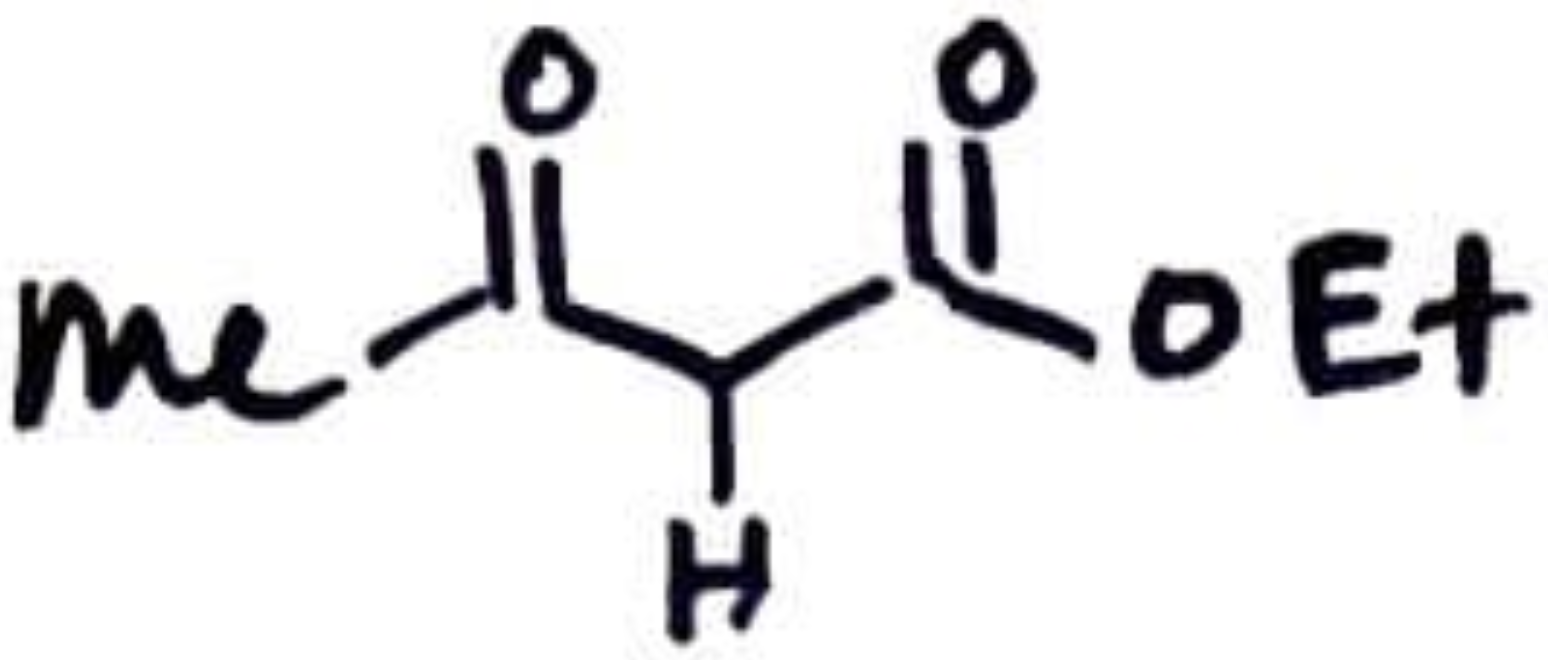
\includegraphics[width=0.15\linewidth]{EtOacac.png}
        \caption{Ethyl acetoacetate.}
        \label{fig:EtOacac}
    \end{figure}
    \begin{itemize}
        \item Here, we have a \emph{ketone} next to an ester group.
        \begin{itemize}
            \item The reason that one is an ethyl ester and the other is a methyl ester is historical; we are totally fine to use ethyl or methyl esters wherever, as long as we're consistent.
        \end{itemize}
        \item $\pKa\approx 11$ for ethyl acetoacetate.
    \end{itemize}
    \item Let's now begin the synthesis.
    \begin{figure}[H]
        \centering
        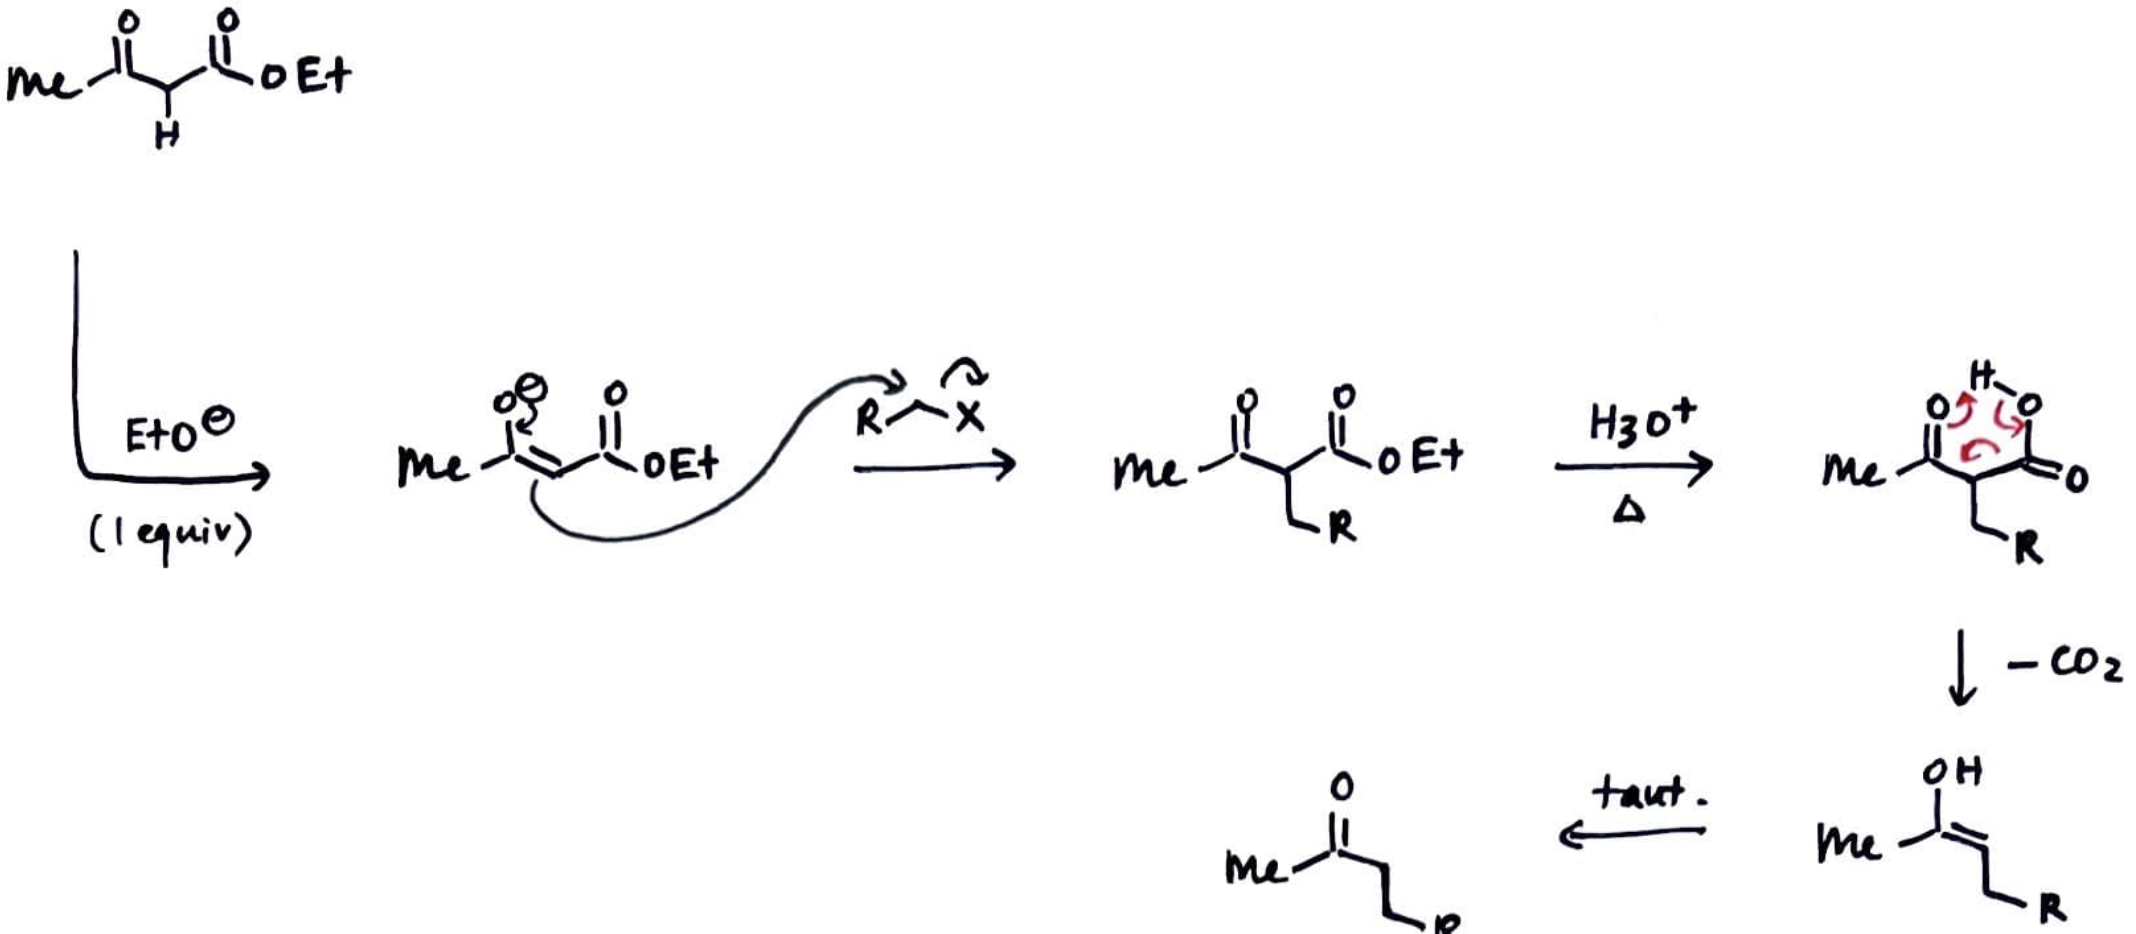
\includegraphics[width=0.9\linewidth]{acacSynth.png}
        \caption{Acetoacetate synthesis.}
        \label{fig:acacSynth}
    \end{figure}
    \begin{itemize}
        \item Adding 1 equivalent of \ce{EtO-} deprotonates to the enolate.
        \begin{itemize}
            \item Note that the resonance will be primarily with the ketone, \emph{not} the ester!
        \end{itemize}
        \item Then we can do our alkylation.
        \begin{itemize}
            \item We could even do a second alkylation, but we're just not going to show that here.
        \end{itemize}
        \item Next step: We heat our intermediate in acid, which first gives ester hydrolysis to the \textbf{$\bm{\beta}$-ketoacid}.
        \begin{itemize}
            \item $\beta$-ketoacids are known to undergo decarboxylation to yield enols!
        \end{itemize}
        \item However, in acidic solution, our enol will quickly tautomerize to a ketone.
        \item Takeaway: This reaction is equivalent to enolate alkylation with LDA (see Figure \ref{fig:enolateKinetic}).
        \begin{itemize}
            \item However, LDA is pyrophoric and hence nasty to work with.
            \item The acetoacetate synthesis, however, is \textbf{bucket chemistry} (easy, safe, and scalable).
        \end{itemize}
    \end{itemize}
    \item TTQ: Make 2-methylhexa-1,5-diene from ethyl acetoacetate, allyl bromide, any other reagent we want with two or fewer carbons, and any other non-carbon reagent.
    \begin{figure}[H]
        \centering
        \begin{subfigure}[b]{\linewidth}
            \centering
            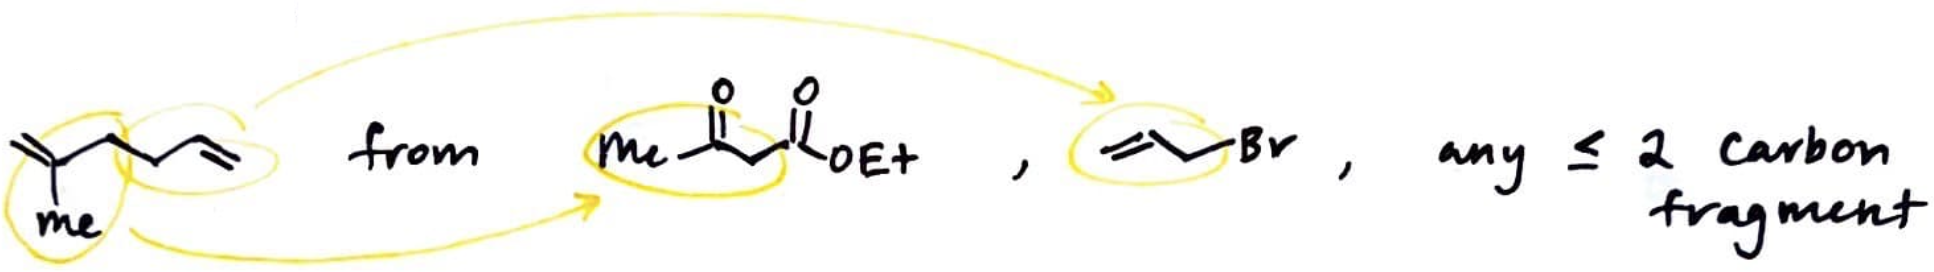
\includegraphics[width=0.75\linewidth]{TTQacaca.png}
            \caption{The desired molecule and starting materials.}
            \label{fig:TTQacaca}
        \end{subfigure}\\[1em]
        \begin{subfigure}[b]{\linewidth}
            \centering
            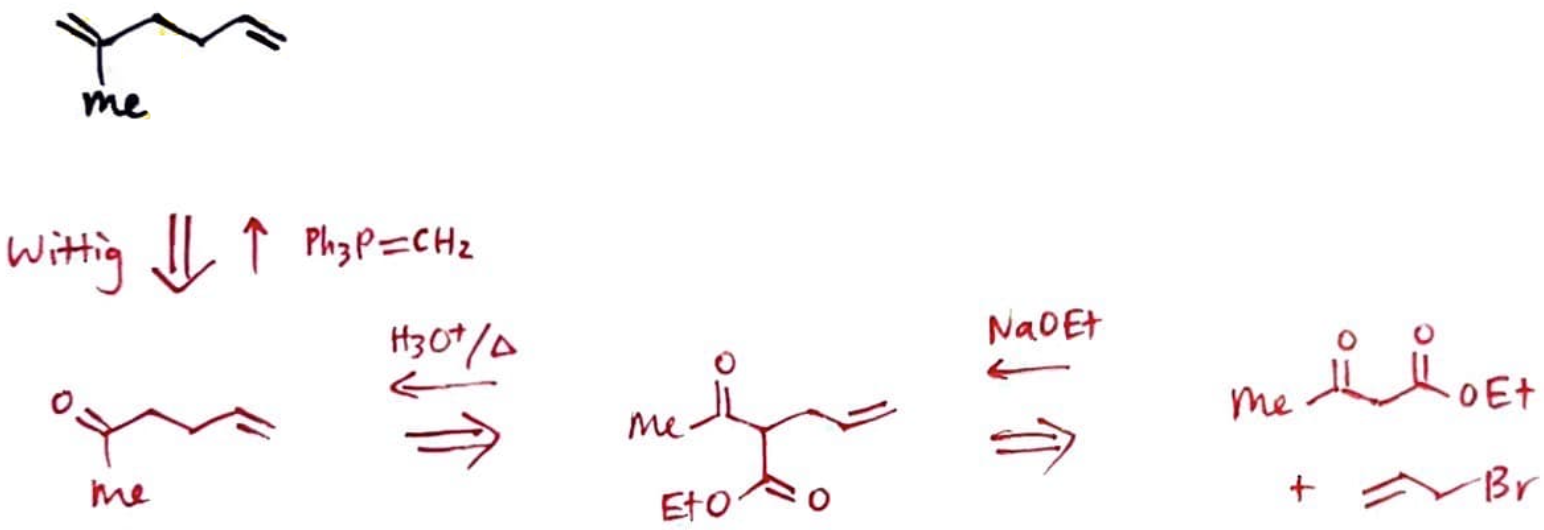
\includegraphics[width=0.65\linewidth]{TTQacacb.png}
            \caption{Retrosynthetic pathway.}
            \label{fig:TTQacacb}
        \end{subfigure}
        \caption{TTQ: Using the acetoacetate synthesis.}
        \label{fig:TTQacac}
    \end{figure}
    \begin{itemize}
        \item Match up the carbons as we've done previously.
        \item A Wittig would yield the product.
        \item Next step: We can go back to the acetoacetate.
        \item Next step: Do alkylation from the starting materials.
    \end{itemize}
\end{itemize}




\end{document}